\documentclass[a4paper]{article}
\usepackage{hyperref}
\usepackage{graphicx}
\usepackage{amsmath,amsfonts,amsmath,amsthm,amssymb}
\usepackage{caption}
\usepackage{multirow}
\usepackage{physics}
\usepackage{tikz}
\usepackage{cleveref}
\usepackage{pgfplotstable}
\usepackage{siunitx}
\usepackage{wrapfig}
\usepackage{graphicx}
\usepackage{subfiles}
\usepackage{bm}
\usepackage{xcolor}
\usepackage[french]{babel}
\usepackage{titlesec}
\usepackage{lmodern}
\usepackage{braket}
\usepackage{geometry}
\usepackage{chngcntr}
 \geometry{
 a4paper,
 total={170mm,257mm},
 left=20mm,
 top=20mm,
 }

\numberwithin{equation}{part}
\counterwithin*{section}{part}

\pgfplotsset{width=10cm,compat=1.16}

\newcommand{\ti}{\times}
\newcommand{\h}{\hbar}
\renewcommand{\d}{\mathrm{d}}


\titleformat{\paragraph}
{\normalfont\normalsize\bfseries}{\theparagraph}{1em}{}
\titlespacing*{\paragraph}
{0pt}{3.25ex plus 1ex minus .2ex}{1.5ex plus .2ex}

\title{\textbf{PHYS-F203 - Introduction à la Mécanique Quantique} \\ \textit{Basé sur les notes de Prof. Serge Massar}}
\author{MOEIL Juian \and ABDUL SATER Sami}
\date{\textbf{Année académique 2020-2021}}

\newtheorem{theorem}{Théorème}[section]
\newtheorem{definition}[theorem]{Définition}
\newtheorem{lemma}[theorem]{Lemme}
\newtheorem{Property}[theorem]{Proposition}
\newtheorem{corollary}[theorem]{Corollaire}
\newtheorem{remark}[theorem]{Remarque}
\newtheorem*{preuve}{Preuve}
\newtheorem{reminder}[theorem]{Rappel théorique}
\newtheorem{exemple}[theorem]{Exemple}

\renewcommand\qedsymbol{$\blacksquare$}

\setcounter{tocdepth}{2}

\begin{document}

\maketitle
\begin{center}
    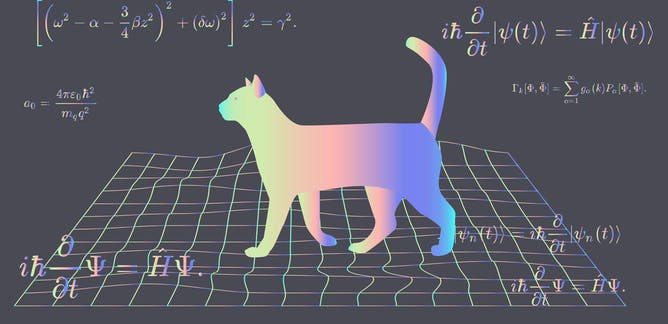
\includegraphics[scale=0.65]{Images/cat.jpg}
\end{center}
\begin{center}
    
\includegraphics[scale=0.2]{Images/sciences.png}
\end{center}
\begin{center}
    
\includegraphics[scale=0.50]{Images/ULB.jpg}
\end{center}

\newpage
\tableofcontents

\newpage
\begin{abstract}
\textit{Ces notes traitent de l'interprétation de Copenhague de la Mécanique Quantique. De plus, le symbôle $\doteq$ sera intensément employé, pour signifier "par définition". Finalement, les vecteurs seront indiqués en gras, selon $\vec{x} \doteq \bm{x}$ Insistons que ces notes ont été rédigées par des étudiant.e.s, et qu'elles contiennent probablement des fautes. N'hésitez pas à contacter $\href{mailto:juian.moeil@ulb.be}{\text{MOEIL Juian}}$} ou $\href{mailto:sami.abdul.sater@ulb.be}{\text{ABDUL SATER Sami}}$. 
\end{abstract}
\subfile{Chapitre 1/chapitre1.tex}
\newpage
\subfile{Chapitre 2/chapitre2.tex}
\newpage
\subfile{Chapitre 3/chapitre3.tex}
\newpage
\subfile{Chapitre 4/chapitre4.tex}
\newpage
\subfile{Chapitre 5/chapitre5.tex}
\newpage
\subfile{Chapitre 6/chapitre6.tex}
\newpage
\subfile{Chapitre 7/Chapitre7.tex}
\newpage
\subfile{Chapitre 8/chapitre8.tex}

\newpage
\subfile{Annexe/annexe.tex}

\end{document}